\subsection*{Modulation}
\begin{multicols*}{4}
    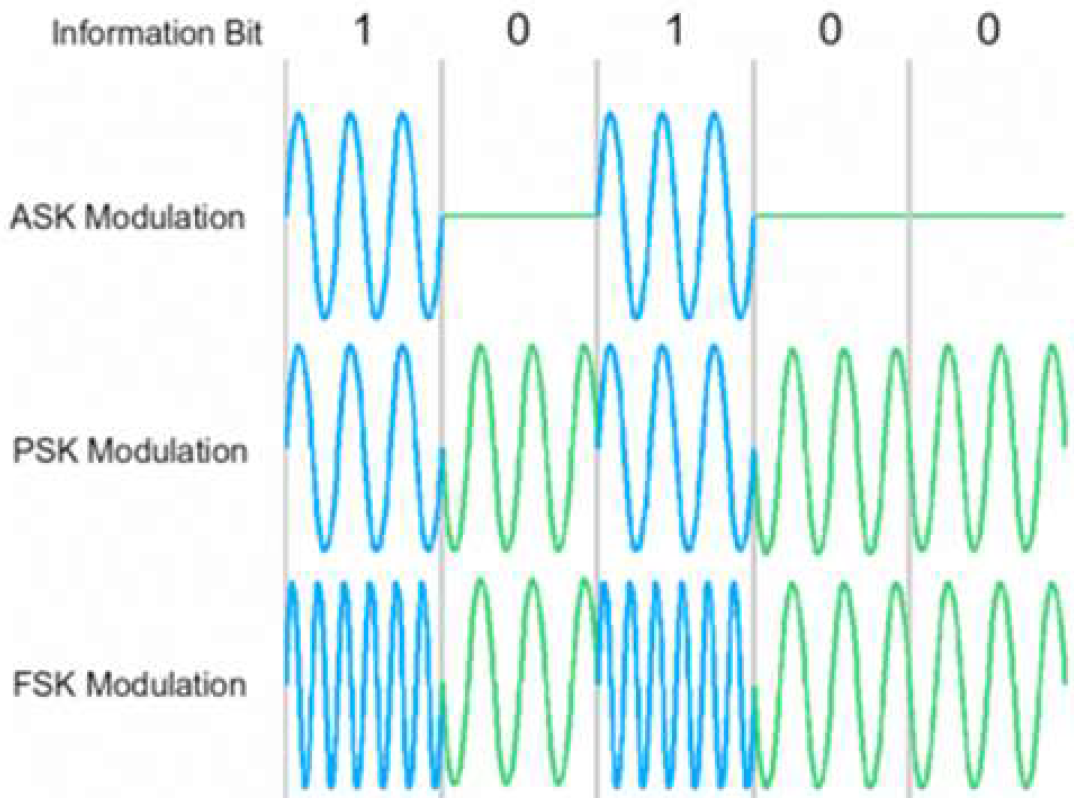
\includegraphics[width=\columnwidth]{images/binary_modulation.png}
    AM: ASK (Amplitude Shift
    Keying)

    PM: PSK (Phase Shift
    Keying) comme on utilise la phase du signal, les nombres complexes sont utilisés.

    FM: FSK (Frequency Shift Keying)

    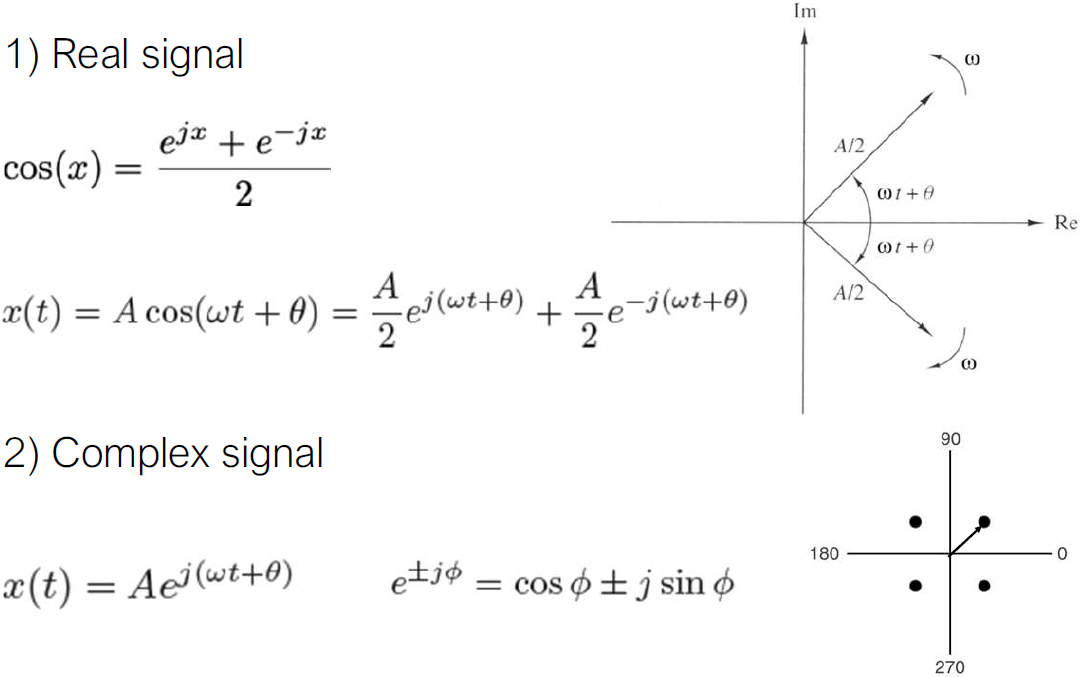
\includegraphics[width=\columnwidth]{images/nombres_complexes.png}
    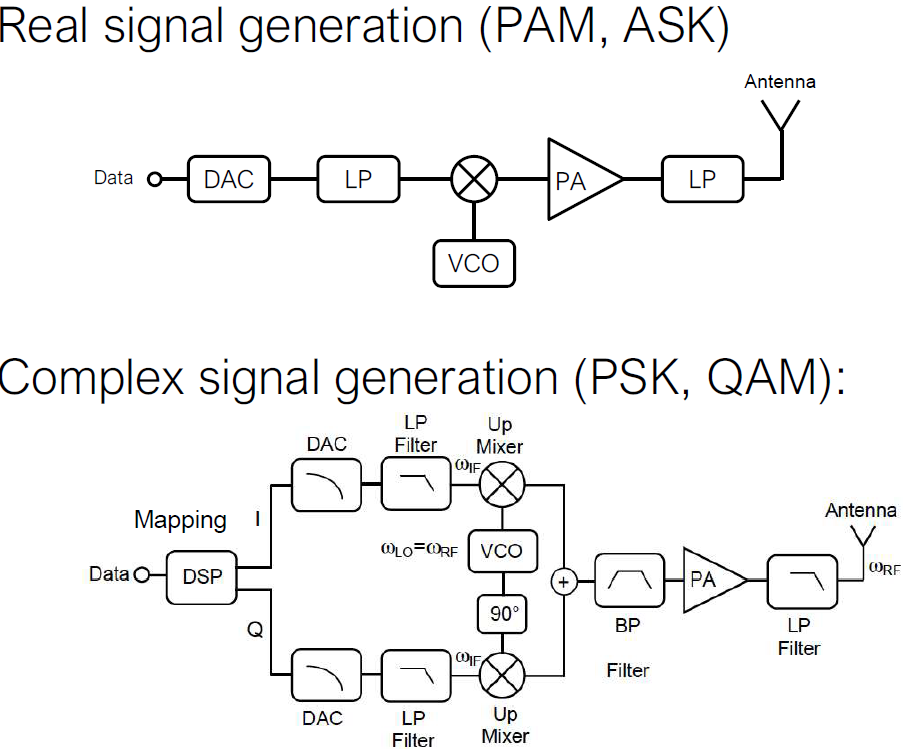
\includegraphics[width=\columnwidth]{images/signal_generation.png}
    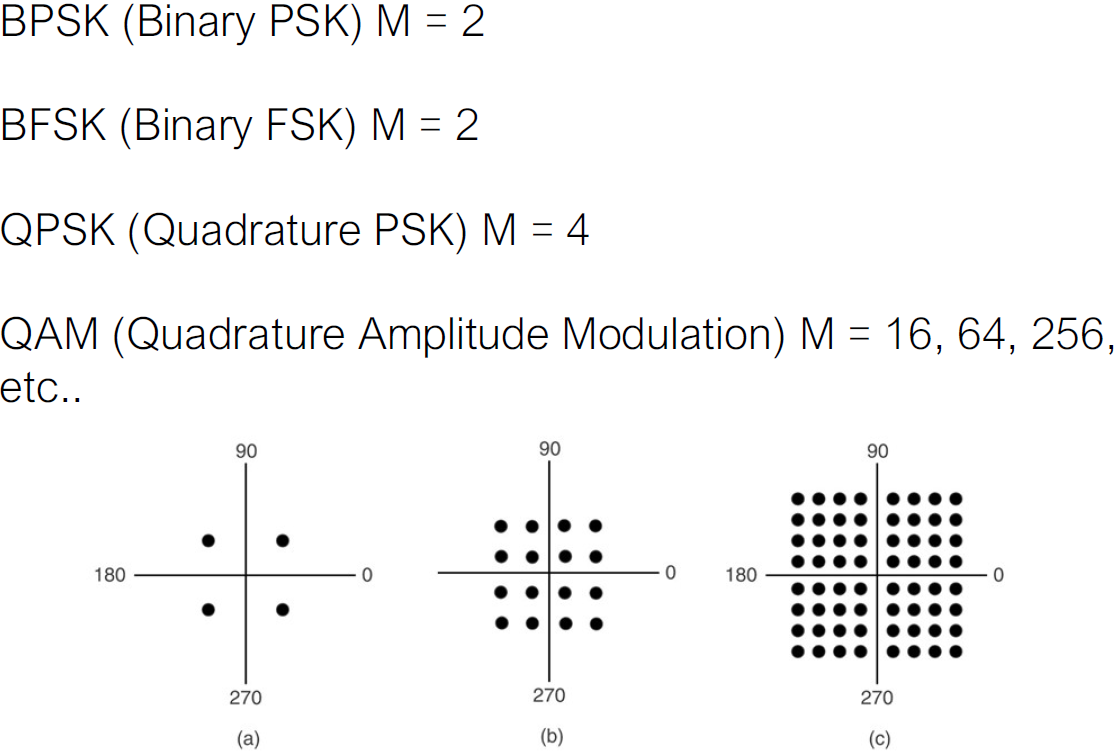
\includegraphics[width=\columnwidth]{images/bfsk_qpsk.png}
    Chaques symboles est représenté par un vecteur dans le plan complexe. La phase du vecteur
    représente le symbole et la norme du vecteur représente l'amplitude du signal.

    Bit energy to noise ratio: Bit energy over noise
    spectral density required for demodulation. It is
    commonly called $E_b/N_0$

    Symbol energy to noise ratio: Symbol energy over
    noise spectral density required for demodulation. It is
    commonly called $E_s/N_0$

    Signal to noise ration : $SNR = \frac{S}{N}=\frac{E_sR}{N_0B}$ where $R_b$ is the bit rate.

    Relation : $\frac{E_s}{N_0}=\frac{E_b}{N_0}\log_2M$

    BER : $\frac{\text{Error count}}{\text{total transmitted bits}}$

    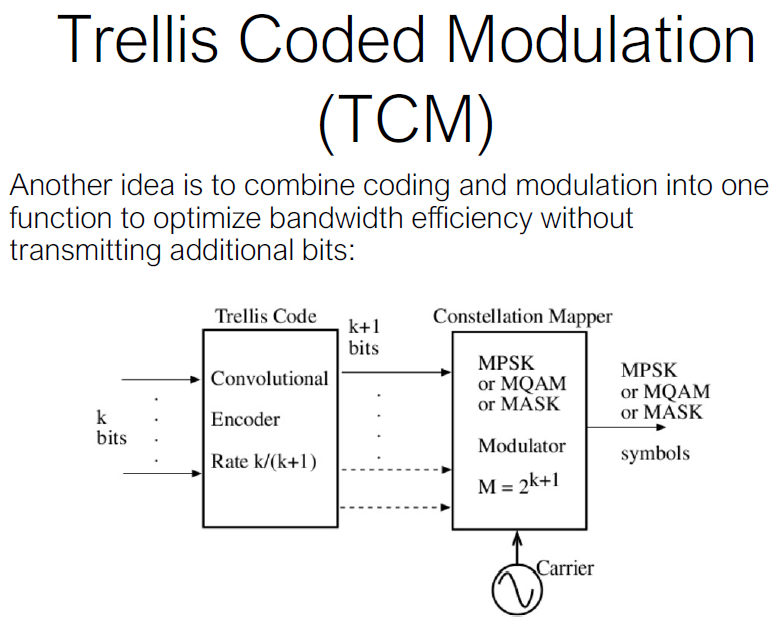
\includegraphics[width=\columnwidth]{images/merde1.png}
    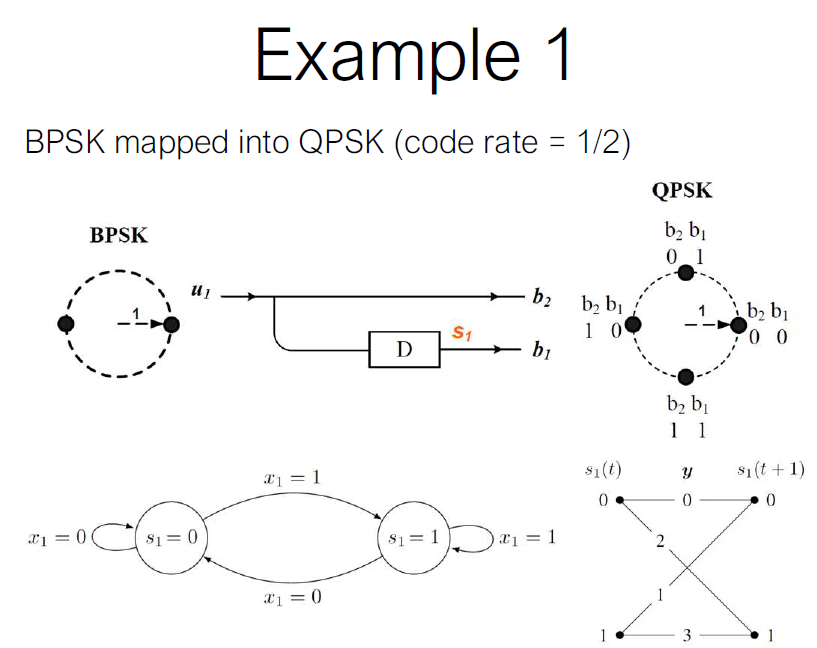
\includegraphics[width=\columnwidth]{images/merde2.png}
    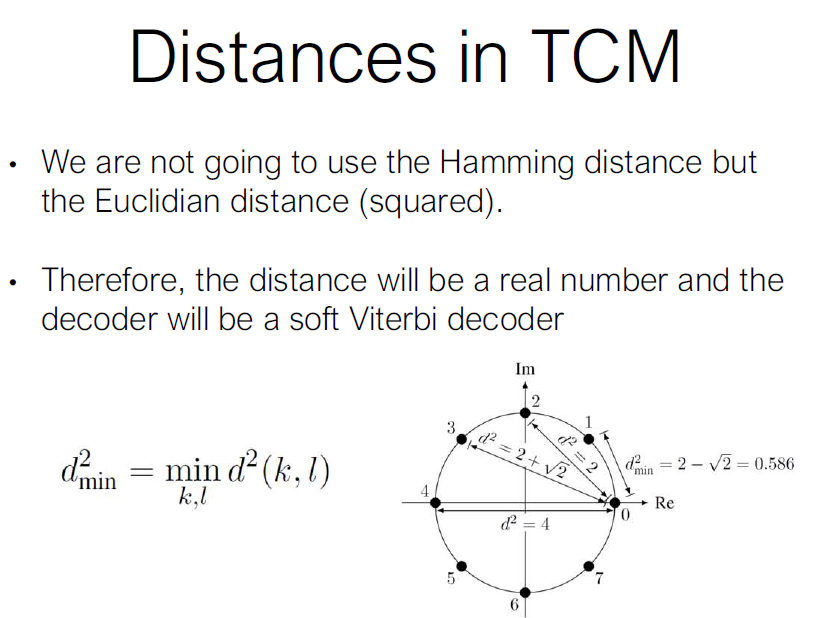
\includegraphics[width=\columnwidth]{images/merde3.png}
    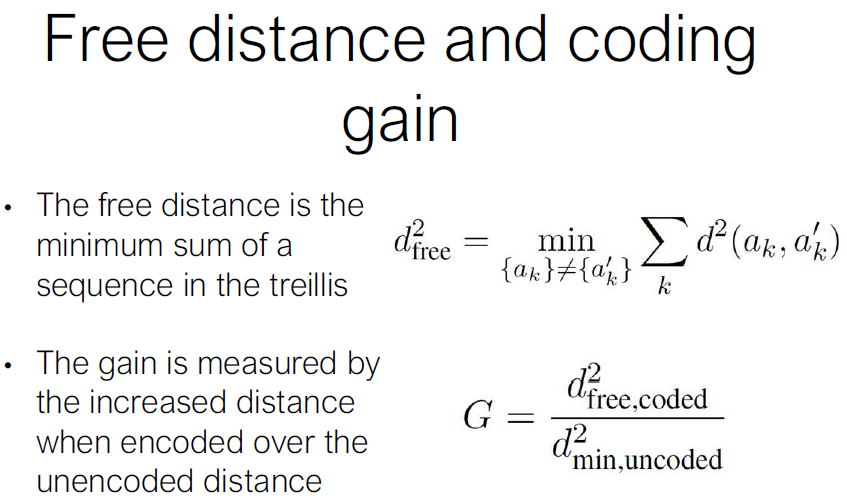
\includegraphics[width=\columnwidth]{images/merde4.png}
    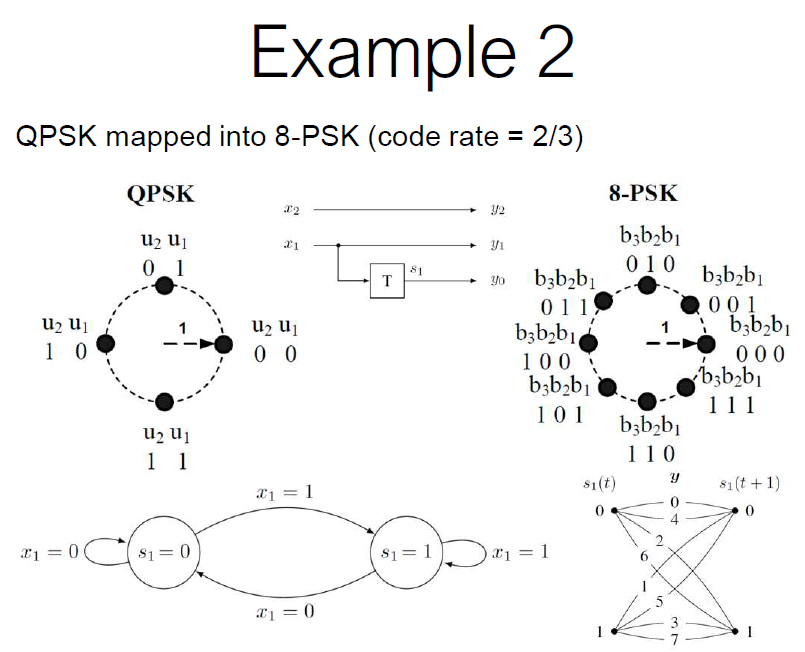
\includegraphics[width=\columnwidth]{images/merde5.png}
    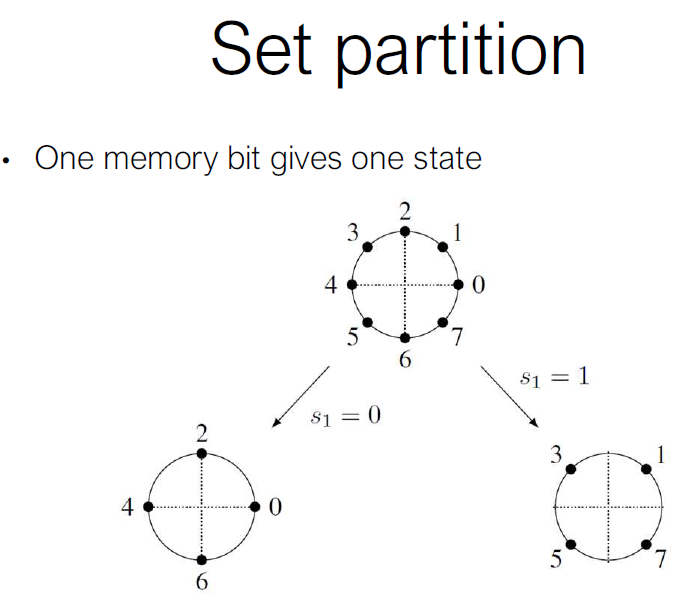
\includegraphics[width=\columnwidth]{images/merde6.png}
    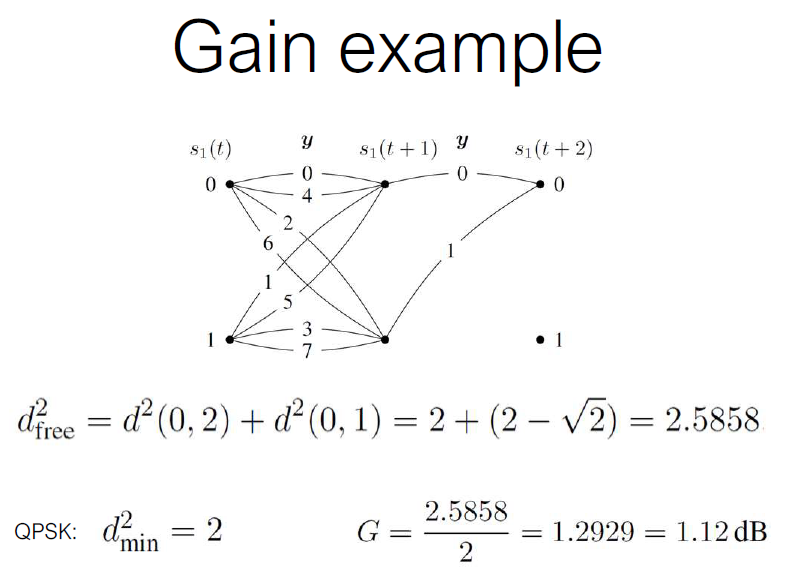
\includegraphics[width=\columnwidth]{images/merde7.png}
    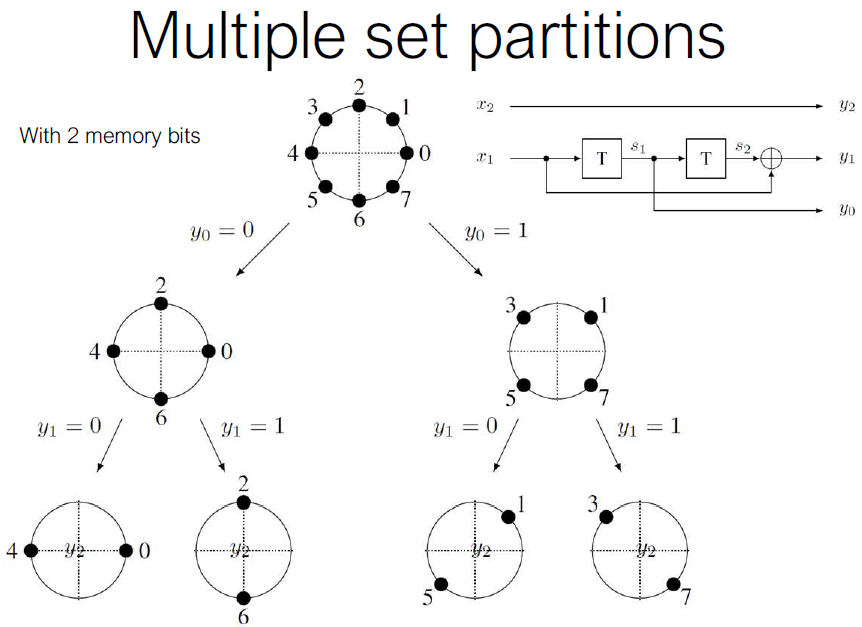
\includegraphics[width=\columnwidth]{images/merde8.png}
    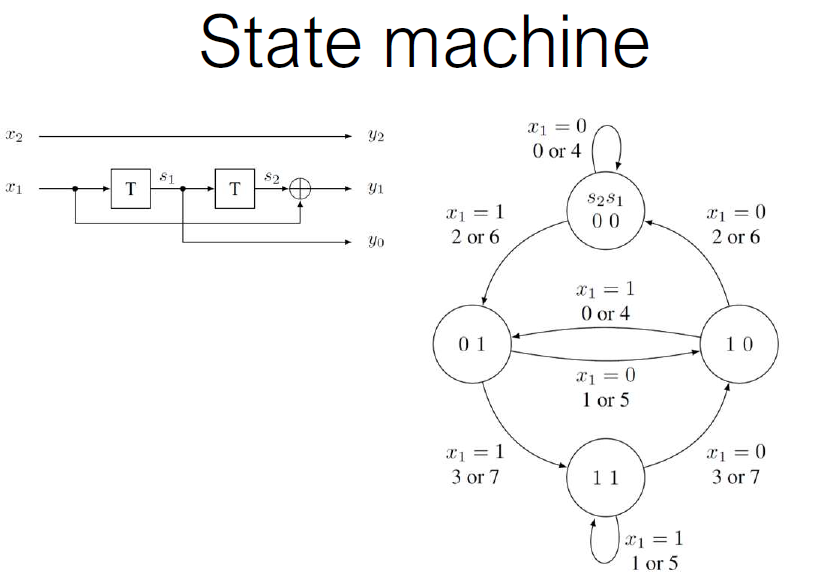
\includegraphics[width=\columnwidth]{images/merde9.png}
    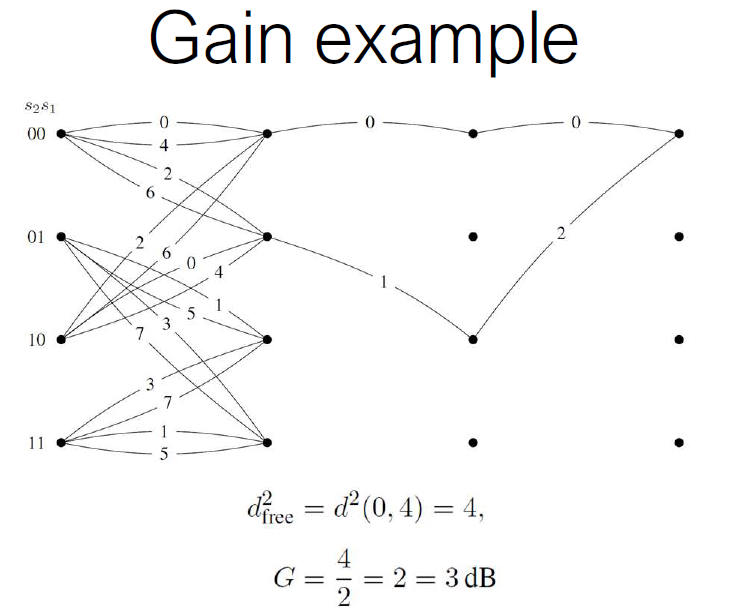
\includegraphics[width=\columnwidth]{images/merde10.png}
\end{multicols*}

